\documentclass[12pt]{ociamthesis}  % default square logo 
%\documentclass[12pt,beltcrest]{ociamthesis} % use old belt crest logo
%\documentclass[12pt,shieldcrest]{ociamthesis} % use older shield crest logo

%load any additional packages
\usepackage{amssymb}
\usepackage{listings}

\usepackage{color}
 
\definecolor{codegreen}{rgb}{0,0.6,0}
\definecolor{codegray}{rgb}{0.5,0.5,0.5}
\definecolor{codepurple}{rgb}{0.58,0,0.82}
\definecolor{backcolour}{rgb}{0.95,0.95,0.92}
 
\lstdefinestyle{mystyle}{
    backgroundcolor=\color{backcolour},   
    commentstyle=\color{codegreen},
    keywordstyle=\color{magenta},
    numberstyle=\tiny\color{codegray},
    stringstyle=\color{codepurple},
    basicstyle=\footnotesize,
    breakatwhitespace=false,         
    breaklines=true,                 
    captionpos=b,                    
    keepspaces=true,                 
    numbers=left,                    
    numbersep=5pt,                  
    showspaces=false,                
    showstringspaces=false,
    showtabs=false,                  
    tabsize=2,
    language=python
}
 
\lstset{style=mystyle}
%input macros (i.e. write your own macros file called mymacros.tex 
%and uncomment the next line)
%\include{mymacros}

\title{Modul Praktikum \\[1ex]     %your thesis title,
        Algoritma}   %note \\[1ex] is a line break in the title

\author{Rolly Maulana Awangga}             %your name
\college{0410118609\\[5ex]
Applied Bachelor of Informatics Engineering}  %your college

%\renewcommand{\submittedtext}{change the default text here if needed}
\degree{Politeknik Pos Indonesia}     %the degree
\degreedate{Bandung 2019}         %the degree date

%end the preamble and start the document
\begin{document}

%this baselineskip gives sufficient line spacing for an examiner to easily
%markup the thesis with comments
\baselineskip=18pt plus1pt

%set the number of sectioning levels that get number and appear in the contents
\setcounter{secnumdepth}{3}
\setcounter{tocdepth}{3}


\maketitle                  % create a title page from the preamble info
\begin{dedication}
`Jika Kamu tidak dapat menahan lelahnya belajar, \\
Maka kamu harus sanggup menahan perihnya Kebodohan.'\\ 
~Imam Syafi'i~\\
\end{dedication}        % include a dedication.tex file
\begin{acknowledgements}
Pertama-tama kami panjatkan puji dan syukur kepada Allah SWT yang telah memberikan rahmat dan hidayah-Nya sehingga Buku Pedoman Tingkat Akhir ini dapat diselesaikan.
\end{acknowledgements}   % include an acknowledgements.tex file
\begin{abstract}
	Buku Pedoman ini dibuat dengan tujuan memberikan acuan, bagi mahasiswa Tingkat Akhir dan dosen
	Pembimbing. Pada intinya buku ini menjelaskan secara lengkap tentang Standar pengerjaan Intership  dan 
	Tugas Akhir
	di Program Studi D4 Teknik Informatika, dan juga mengatur mekanisme, teknik penulisan, serta
	penilaiannya.Dengan demikian diharapkan semua pihak yang terlibat dalam aktivitas Bimbingan Mahasiswa Tingkat Akhir
	berjalan lancar dan sesuai dengan standar.
\end{abstract}          % include the abstract

\begin{romanpages}          % start roman page numbering
\tableofcontents            % generate and include a table of contents
\listoffigures              % generate and include a list of figures
\end{romanpages}            % end roman page numbering

%now include the files of latex for each of the chapters etc
\chapter{Python}
Python merupakan bahasa pemrograman tingkat tinggi yang diracik oleh Guido van Rossum.

Python banyak digunakan untuk membuat berbagai macam program, seperti: program CLI, Program GUI (desktop), Aplikasi Mobile, Web, IoT, Game, Program untuk Hacking, dsb.

Python juga dikenal dengan bahasa pemrograman yang mudah dipelajari, karena struktur sintaknya rapi dan mudah dipahami.
 \section{Hello World Python}
 \subsection{Teori}
 Python memang sangat sederhana dibandingkan bahasa yang lainnya. Tidak perlu ini dan itu untuk membuat program Hello World!.
Bahkan tagline di websitenya menjelaskan, kalau python akan membuatmu bekerja lebih cepat dan efektif.
Berikut salah satu contoh dasar perbedaan python dengan bahasa pemograman lain:
\par\textbf{C++ "Hello World"}
\begin{lstlisting}
#include <iostream.h>
main()
{
count << "hello world!";
}
retun 0
\end{lstlisting}
\par \textbf{Java "Hello World"}
\begin{lstlisting}
class HelloWorldApp
{
public static void main(String[] args)
    {
    System.out.printin("Hello World!");
    }
}
\end{lstlisting}
\par \textbf{Python}
\begin{lstlisting}
print "Hello World"
\end{lstlisting}


\chapter{Fungsi Pada Python}
\par Pada pembuatan program yang kompleks dan memiliki banyak fitur, kita diharuskan menggunakan fungsi. hal tersebut karena bisa jadi kita akan kerepotan menulis kode programnya, karena banyak yang harus ditulis dan kode akan menjadi sulit dibaca dan dirawat (maintenance).
\par Dengan fungsi, kita dapat memecah program besar menjadi sub program yang lebih sederhana. Masing-masing fitur pada program dapat kita buat dalam satu fungsi. Pada saat kita membutuhkan fitur tersebut, kita tinggal panggil fungsinya saja.Hal ini akan kita coba pada contoh program yang sudah saya sediakan di bawah.Namun, terlebih dahulu. Kita harus memahami teori dasar dan hal apa saja yang harus kita ketahui tentang fungsi di Python.
\section{Cara Membuat Fungsi Python}
Fungsi pada Python, dibuat dengan kata kunci def kemudian diikuti dengan nama fungsinya.

Contoh: 
\lstinputlisting[language=Python, breaklines=true, caption=koding]{src/1.py}
 Sama seperti blok kode yang lain, kita juga harus memberikan identasi (tab atau spasi 2x) untuk menuliskan isi fungsi.
\newpage \begin{figure}[!htbp]
    \centering
    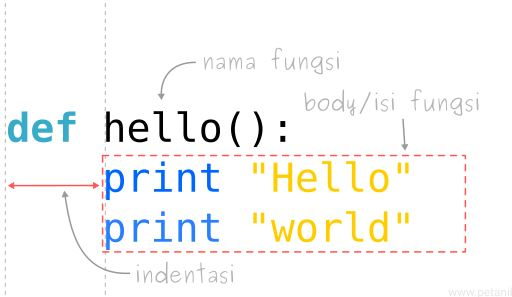
\includegraphics[scale=0.5]{figures/p2}
    \label{fungsi}
\end{figure}
\par Setelah kita buat, kita bisa memanggilnya seperti ini:
\lstinputlisting[language=Python, breaklines=true, caption=koding]{src/5.py}
Sebagai contoh, coba tulis kode program berikut:
\lstinputlisting[language=Python, breaklines=true, caption=koding]{src/6.py}
Hasilnya:
\lstinputlisting[language=Python, breaklines=true, caption=koding]{src/7.py}
Intinya adalah apapun yang ada di dalam fungsi, ketika dipanggil itulah yang akan dilakukan.
\par FYI: fungsi juga dapat dipanggil pada fungsi lain, bahkan bisa memanggil dirinya sendiri. Fungsi yang memanggil dirinya sendiri, disebut fungsi rekursif.
\section{Fungsi Dengan Parameter}
\par Fungsi parameter merupakan variabel yang menampung nilai untuk diproses di dalam fungsi.
\par \textbf{Contoh}:
\lstinputlisting[language=Python, breaklines=true, caption=koding]{src/8.py}
Pada contoh diatas, kita membuat fungsi dengan parameter ucapan.Kemudian cara untuk pemanggilan fungsi yang memiliki parameter tersebut adalah seperti berikut:
\lstinputlisting[language=Python, breaklines=true, caption=koding]{src/9.py}
"Selamat siang" adalah nilai parameter yang kita berikan.
\par Untuk parameter yang lebih dari satu kita bisa menggunakan tanda koma (,) untuk memisahnya.
\par\textbf{Contoh}:

\lstinputlisting[language=Python, breaklines=true, caption=koding]{src/namafile.py}

\par\textbf{Hasilnya}:
\lstinputlisting[language=Python, breaklines=true, caption=koding]{src/10.py}
\section{Fungsi Yang Mengembalikan Nilai}
Fungsi yang tidak mengembalikan nilai biasanya disebut dengan prosedur.
Tetapi, suatu waktu kita butuh hasil proses dari fungsi untuk digunakan pada proses berikutnya.Maka fungsi harus mengembalikan nilai dari hasil pemrosesannya.Cara mengembalikan nilai adalah menggunakan kata kunci \textit{return} lalu diikuti dengan nilai atau \textit{variabel} yang akan dikembalikan.
\par\textbf{Contoh}:
\lstinputlisting[language=Python, breaklines=true, caption=koding]{src/11.py}
\par \textbf{Hasilnya}:
\lstinputlisting[language=Python, breaklines=true, caption=koding]{src/12.py}
Perbedaan dengan fungsi luas segitiga() yang sebelumnya adalah pada fungsi luas segitiga() kita melakukan print dari hasil pemrosesan secara langsung di dalam fungsinya. Sedangkan fungsi luas persegi(), kita melakukan print pada saat pemanggilannya.Jadi, fungsi luas persegi() akan bernilai sesuai dengan hasil yang dikembalikan.
Sehingga kita dapat memanfaatkannya untuk pemerosesan berikutnya.
\par\textbf{Seperti pada contoh berikut}:
\lstinputlisting[language=Python, breaklines=true, caption=koding]{src/13.py}
\par Pada contoh di atas, kita melakukan pemanggilan fungsi luas persegi() untuk menghitung volume persegi.
\section{Variabel Global dan Lokal pada Python}
\par Variabel Global(berbeda file) adalah variabel yang bisa diakses dari semua fungsi, sedangkan variabel lokal(satu file) hanya bisa diakses di dalam fungsi tempat ia berada saja.Pada Python, urutan pengaksesan variabel (scope) dikenal dengan sebutan LGB (Local, Global, dan Build-in).Jadi program python mulai mencari vairabel lokal terlebih dahulu, kalau ada maka itu yang digunakan.Tetapi kalau tidak ada, pencarian terus ke Global, dan Build-in. Variabel Build-in adalah variabel yang sudah ada di dalam Python.
\par\textbf{Contoh program}:
\lstinputlisting[language=Python, breaklines=true, caption=koding]{src/14.py}
\par \textbf{Hasilnya}:
\lstinputlisting[language=Python, breaklines=true, caption=koding]{src/15.py}
\newpage Perhatikanlah variabel nama yang berada di dalam fungsi help() dan diluar fungsi `help(). Variabel nama yang berada di dalam fungsi help() adalah variabel lokal. Jadi, saat kita memanggil fungsi help() maka nilai yang akan tampil adalah nilai yang ada di dalam fungsi help(). Mengapa yang tampil tidak global di karenakan Python mulai mencari dari lokal, ke global, dan build-in. Jika di tiga tempat itu tidak ditemukan, maka biasanya akan terjadi NameError atau variabel tidak ditemukan.

\section{Contoh Program Dengan fungsi}
Berikut adalah langkah membuat program nya. Silahkan buat file baru bernama programfungsi.py. Lalu kita mulai tulis kodenya. Pertama kita buat sebuah variabel global berupa list untuk menampung judul-judul buku.
\lstinputlisting[language=Python, breaklines=true, caption=koding]{src/16.py}
Kemudian program ini akan mampu melakukan operasi CRUD (Create, Read, Update, dan Delete). Maka kita membutuhkan fungsi-fungsi berikut:
\lstinputlisting[language=Python, breaklines=true, caption=koding]{src/17.py}
\par \textbf{Langkah Berikutnya adalah dimulai dari fungsi show\_data()}:
\lstinputlisting[language=Python, breaklines=true, caption=koding]{src/18.py}
Fungsi di atas akan mengecek isi dari list buku. Jika isinya kosong (len(buku) <= 0) maka tampilkan "BELUM ADA DATA". Namun, apabila ada isinya, maka tampilkan semua isinya dengan perulangan.
\par\textbf{Selanjutnya membuat fungsi insert\_data()}:

\lstinputlisting[language=Python, breaklines=true, caption=koding]{src/19.py}
\par\textbf{Selanjutnya membuat fungsi edit\_data()}:
\lstinputlisting[language=Python, breaklines=true, caption=koding]{src/20.py}
Fungsi di atas akan menampilkan isi dari list buku dengan memanggil fungsi show\_data() di dalamnya. Setelah itu, kita meminta user untuk menginputkan ID atau nomer indeks buku yang akan diedit. Lalu kita lakukan pengecekan, jika ID yang diinputkan melebihi dari isi list buku (indeks > len(buku)), maka tampilkan pesan "ID salah". Namun, apabila tidak melebihi dari isi buku, maka ambil input untuk judul baru dan simpan sesuai ID-nya.
\par \textbf{Selanjutnya membuat fungsi delete\_data()}:
\lstinputlisting[language=Python, breaklines=true, caption=koding]{src/21.py}
Hampir sama dengan fungsi edit\_data(). Fungsi delete\_data() juga harus menampilkan isi list buku dan mengambil ID yang akan dihapus. Kita dapat menghapus item pada list dengan fungsi remove().
 \par Setelah langkah di atas, ada 2 fungsi lagi yang di butuhkan:
 \begin{enumerate}
     \item Fungsi untuk menampilkan menu
     \item Fungsi untuk keluar (sudah ada di python: exit())
 \end{enumerate}
\lstinputlisting[language=Python, breaklines=true, caption=koding]{src/22.py}
Fungsi di atas akan menampilkan menu dari 1–5, lalu memanggil fungsi-fungsi yang sudah dibuat berdasarkan menu yang dipilih.

Terakhir, kita harus membuat main loop programnya.
\lstinputlisting[language=Python, breaklines=true, caption=koding]{src/23.py}
Program akan mengulang terus-menerus sampai fungsi exit() dieksekusi.

if \_\_name\_\_ == "\_\_main\_\_": adalah blok main di Python. Sebenarnya tanpa ini, programnya sudah bisa dijalankan namun agar lebih bagus kita baiknya menambahkannya.
\par\textbf{Sehingga kode lengkapnya akan seperti ini}:
\lstinputlisting[language=Python, breaklines=true, caption=koding]{src/24.py}
\chapter{Class Pada Phyton}
\par Class merupakan sebuah objek yang di dalam nya biasanya terdapat beberapa metode yang memang merupakan isi dari sebuah class ini. Class dan metode ini biasa di sembut sebagai OOP atau object oriented programing. Dan OOP ini memang fungsinya untuk memudahkan proses atau kegiatan programing kita. Class ini merupakan sebuah objek yang lebih complex dengan di dalamnya berisi beberapa metode.
\section{Cara Membuat Sebuah Class Pada Python}
Untuk membuat sebuah class ini, harus kita awali dengan sebuah kata kunci. Yaitu “class” yang kemudian di ikuti dengan “nama class nya”. Dan yang terakhir adalah tanda kurung buka dan tutup serta tanda titik dua “()” dan ‘:’.  untuk lebih mudahnya kita bisa lihat atau simak contohnya di bawah ini:
\lstinputlisting[language=Python, breaklines=true, caption=koding]{src/25.py}
\newpage \section{Cara memanggil sebuah class dan metode didalamnya.}
Untuk memanggil sebuah class, sama saja seperti layak nya memanggil metode.. Kita cukup menyebutkan nama classnya dengan di akhiri dengan tanda kurung buka dan tutup seperti di bawah ini.
\lstinputlisting[language=Python, breaklines=true, caption=koding]{src/26.py}
Untuk memanggil metodenya, kita cukup menggunakan memanggil class yang kemudian di ikuti dengan pemanggilan nama metode yang tersedia di dalam class tersebut dengan di pisahkan oleh tanda titik. Seperti di bawah ini.
\lstinputlisting[language=Python, breaklines=true, caption=koding]{src/27.py}
Untuk memudahkan pemanggilan metode ini, kita bisa menampung class nya ke dalam sebuah variabel terlebih dahulu. Yang kemudian kita panggil metodenya seperti di bawah ini.
\lstinputlisting[language=Python, breaklines=true, caption=koding]{src/28.py}
Di dalam sebuah class,biasanya terdapat sebuah metode yang namanya sudah di sediakan oleh python. Namanya adalah “\_\_init\_\_”. Dan jika contoh di atas kita tambahkan \_\_init\_\_ maka kurang lebih akan seperti berikut ini.
\lstinputlisting[language=Python, breaklines=true, caption=koding]{src/29.py}
Dan sama seperti metode, kita bisa menggunakan atau mengirim sebuah nilai di dalamnya atau tidak. Untuk mengirimnya sama saja. Kita cukup memasukkan sebuah variabel di dalam tanda Kurung pada metode \_\_init\_\_. Dan ingat, bukan pada tanda kurung milik clannya ya. Seperti dibawah ini:
\lstinputlisting[language=Python, breaklines=true, caption=koding]{src/30.py}
Untuk memanggil sebuah class yang memiliki parameter, tentu kita harus memasukkan sebuah nilai saat pemanggilannya. Seperti yang ada di bawah ini.
\lstinputlisting[language=Python, breaklines=true, caption=koding]{src/31.py}
Penjelasan mengenai \_\_init\_\_, metode ini merupakan metode yang akan langsung dijalankan ketika class kita di panggil nantinya. Jadi kita tidak perlu memanggil metodenya secara manual seperti metode - metode yang lain seperti yang sudah saya jelaskan di atas.
\section{Contoh dan pemanfaatan sebuah class pada python.}
Setelah kita mengetahui cara membuat dan cara memanggilnya, maka sekarang saya akan mencoba untuk melihat contoh dan pemanfaatan dari sebuah class ini. Hal ini tentu agar membuat lebih paham mengenai apa yang dimaksud dengan class pada python ini. Contoh programnya di seperti bawah ini:
\lstinputlisting[language=Python, breaklines=true, caption=koding]{src/32.py}

\chapter{Import}
\section{Import File dalam folder}
\par Bagi yang sudah berpengalaman terjun di dunia computer programming, mereka sudah biasa mengelola banyak file kode. Tentunya banyak file program yang kita temui tidak hanya memiliki satu file script saja. Mereka memisahkan script fungsi ataupun class untuk mempermudah debug, refactor code dan memperjelas struktur kode mereka. Cara ini disebut dengan Modularisasi. Hal yang sangat saya rasakan dari keuntungan modularisasi ini adalah kita menjadi tidak perlu mengubah banyak kode untuk hal pengembangan atau perubahan sistem program kita. Di python, cara meng-import file nya terdapat banyak cara. Namun kita akan menggunakan cara yang lebih sederhana dan mudah.
\subsection{Cara import dalam direktori yang sama.}
Misalkan kita sedang berada di direktori kerja bernama ‘project’. Kita memiliki suatu program utama bernama ‘Main.py’ dan file lain bernama ‘KumpulanFungsi.py’. Susunannya seperti ini:
\begin{lstlisting}
- project
  |____ Main.py
  |____ KumpulanFungsi.py
\end{lstlisting}
\par \textbf{Di dalam script KumpulanFungsi.py berisi:}
\begin{lstlisting}
def perkalian(x,y):
   return x * y

def pembagian(x,y):
   return x / y

def pertambahan(x,y):
   return x + y

def pengurangan(x,y):
   return x - y
\end{lstlisting}
\par\textbf{Untuk menggunakan fungsi-fungsi di Main.py, maka cara importnya adalah seperti ini}:
\begin{lstlisting}
#Cara import seluruh isi file
from KumpulanFungsi import *

print pertambahan(10,12)
print pengurangan(20,9)
print pembagian(21,3)
print perkalian(6,6)
\end{lstlisting}
\par \textbf{Atau mengimport function/class yang dibutuhkan saja, untuk tujuan menghemat memori atau membatasi proses yang tidak dibutuhkan. Cara nya seperti ini}:
\begin{lstlisting}
#Cara import satuan function/class
from KumpulanFungsi import pertambahan

print pertambahan(21,24)

#Cara import beberapa function/class
from KumpulanFungsi import perkalian, pembagian

print pertambahan(perkalian(2,2),pembagian(12,3))
\end{lstlisting}
\subsection{Cara import di direktori yang berbeda}
Untuk import dari direktori yang berbeda, python membutuhkan suatu file kosong bernama \_\_init\_\_.py’ di dalam direktori yang berisi file yang akan digunakan. Masih di kasus sebelumnya, kita menambahkan suatu folder baru bernama KumpulanKelas, yang berisi file ‘Kucing.py’ dan ‘Ayam.py’. Maka susunannya akan seperti ini:
\begin{lstlisting}
- project
  |____ KumpulanKelas
        |____ Kucing.py
        |____ Ayam.py
        |____ __init__.py
  |____ Main.py
  |____ KumpulanFungsi.py
\end{lstlisting}
\par \textbf{File Kucing.py berisi}:
\begin{lstlisting}
class Kucing(object):
   def suara(self):
       print "Meow!"
   def jenis(self):
       print "Mamalia"
\end{lstlisting}
\par \textbf{File Ayam.py berisi }:
\begin{lstlisting}
class Ayam(object):
   def suara(self):
      print "Kukuruyuk!"
   def jenis(self):
      print "Unggas"
\end{lstlisting}
\par\textbf{Maka cara importnya seperti berikut}:
\begin{lstlisting}
#Cara import semua function/kelas dari file di direktori lain
from KumpulanKelas.Kucing import *

Morganisa = Kucing()
Morganisa.suara()
Morganisa.jenis()

#Cara import satu function/kelas dari file di direktori lain
from KumpulanKelas.Ayam import Ayam

Pelung = Ayam()
Pelung.suara()
Pelung.jenis()
\end{lstlisting}
Dari kode di atas, from KumpulanKelas.Kucing dimaksud dengan susunan direktori dari terluar sampai nama file yang ingin digunakan.
\newpage \section{Import Library}
\textbf{Berikut 5 library data scientist:}
\begin{enumerate}
    \item \textbf{Scipy}
   \par Kegunaanya adalah untuk menangani operasi aljabar dan matriks serta operasi matematika lainya. Disini kamu dapat menangani sejumlah operasi matematika yang lebih kompleks daripada menggunakan library math bawaan Python. Ada juga beberapa fungsi statistika dasar yang dimiliki oleh Scipy.
    \begin{lstlisting}
>>> import numpy as np
>>> from scipy import linalg
>>> A = np.array([[1,2],[3,4]])
>>> A
array([[1, 2],
      [3, 4]])
>>> linalg.inv(A)
array([[-2. ,  1. ],
      [ 1.5, -0.5]])
>>> b = np.array([[5,6]]) #2D array
>>> b
array([[5, 6]])
>>> b.T
array([[5],
      [6]])
>>> A*b #not matrix multiplication!
array([[ 5, 12],
      [15, 24]])
>>> A.dot(b.T) #matrix multiplication
array([[17],
      [39]])
>>> b = np.array([5,6]) #1D array
>>> b
array([5, 6])
>>> b.T  #not matrix transpose!
array([5, 6])
>>> A.dot(b)  #does not matter for multiplication
array([17, 39])
2. Numpy
\end{lstlisting}
\item \textbf{Numpy}
\par Numpy memiliki kegunaan untuk operasi vektor dan matriks. Fiturnya hampir sama dengan MATLAB dalam mengelola array dan array multidimensi. Numpy merupakan salah satu library yang digunakan oleh library lain seperti Scikit-Learn untuk keperluan analisis data.
\begin{lstlisting}
>>> x = np.array([[1, 2, 3], [4, 5, 6]], np.int32)
>>> type(x)
<type 'numpy.ndarray'>
>>> x.shape
(2, 3)
>>> x.dtype
dtype('int32')
\end{lstlisting}
\item \textbf{Pandas}
\par Dengan menggunakan sistem dataframe, kamu dapat memuat sebuah file ke dalam tabel virtual ala spreadsheet dengan menggunakan Pandas. Dengan menggunakan Pandas, kamu dapat mengolah suatu data dan mengolahnya seperti join, distinct, group by, agregasi, dan teknik seperti pada SQL. Hanya saja dilakukan pada tabel yang dimuat dari file ke RAM.

Pandas juga dapat membaca file dari berbagai format seperti .txt, .csv, .tsv, dan lainnya. Anggap saja Pandas adalah spreadsheet namun tidak memiliki GUI dan punya fitur seperti SQL.
\begin{lstlisting}
import pandas as pd
pd.set_option('display.mpl_style', 'default') # Make the graphs a bit prettier
figsize(15, 5)
broken_df = pd.read_csv('../data/bikes.csv')
# Look at the first 3 rows
broken_df[:3]
\end{lstlisting}
\item \textbf{Matplotlib}
\par Data yang kita olah tentu tidak elok apabila ditampilkan begitu saja dengan tabel hitam saja kepada investor atau manajemen. Bila ditampilkan dengan sejumlah grafik berwarna pasti mereka akan lebih tertarik melihatnya. Matplotlib membantu kamu untuk memvisualisasikan data dengan lebih indah dan rapi.

Ada plot untuk menampilkan data secara 2D atau 3D. Sehingga kamu dapat menampilkan data yang telah kamu olah sesuai kebutuhan. Matplotlib pun terintegrasi dengan iPython Notebook atau Jupyter dimana kamu dapat membuat sebuah buku interaktif yang dapat diberi penjelasan dan kode yang disisipkan begitupun hasil plottingnya.

Matplotlib adalah library paling banyak digunakan oleh data science untuk menyajikan datanya ke dalam visual yang lebih baik.
\begin{lstlisting}
import matplotlib.pyplot as plt
plt.plot([1,2,3,4])
plt.ylabel('some numbers')
plt.show()
\end{lstlisting}
\item \textbf{Scikit-Learn}
\par Machine learning ada yang berbasis statistika ada juga yang tidak. Salah satunya adalah support vector machine dan regresi linier. Mungkin bagi sebagian orang sudah biasa menulis sendiri library untuk implementasi kedua algoritma tadi. Tapi untuk membuatnya dalam waktu singkat tentu butuh waktu yang tidak sedikit pula.

Scikit-Learn memberikan sejumlah fitur untuk keperluan data science seperti:

Algoritma Regresi
Algoritma Naive Bayes
Algoritma Clustering
Algoritma Decision Tree
Parameter Tuning
Data Preprocessing Tool
Export / Import Model
Machine learning pipeline
dan lainnya
Scikit-Learn sudah teruji dan memiliki dokumentasi yang super lengkap. Bahkan kontributornya pun banyak. Scikit-Learn pun menyediakan ekstensi untuk fuzzy logic dan computer vision.
 \begin{lstlisting}
$ python
>>> from sklearn import datasets
>>> iris = datasets.load_iris()
>>> digits = datasets.load_digits()
>>> print(digits.data)  
[[  0.   0.   5. ...,   0.   0.   0.]
 [  0.   0.   0. ...,  10.   0.   0.]
 [  0.   0.   0. ...,  16.   9.   0.]
 ...,
 [  0.   0.   1. ...,   6.   0.   0.]
 [  0.   0.   2. ...,  12.   0.   0.]
 [  0.   0.  10. ...,  12.   1.   0.]]
>>> digits.target
array([0, 1, 2, ..., 8, 9, 8])
>>> digits.images[0]
array([[  0.,   0.,   5.,  13.,   9.,   1.,   0.,   0.],
       [  0.,   0.,  13.,  15.,  10.,  15.,   5.,   0.],
       [  0.,   3.,  15.,   2.,   0.,  11.,   8.,   0.],
       [  0.,   4.,  12.,   0.,   0.,   8.,   8.,   0.],
       [  0.,   5.,   8.,   0.,   0.,   9.,   8.,   0.],
       [  0.,   4.,  11.,   0.,   1.,  12.,   7.,   0.],
       [  0.,   2.,  14.,   5.,  10.,  12.,   0.,   0.],
       [  0.,   0.,   6.,  13.,  10.,   0.,   0.,   0.]])
>>> from sklearn import svm
>>> clf = svm.SVC(gamma=0.001, C=100.)
>>> clf.fit(digits.data[:-1], digits.target[:-1])  
SVC(C=100.0, cache_size=200, class_weight=None, coef0=0.0,
  decision_function_shape='ovr', degree=3, gamma=0.001, kernel='rbf',
  max_iter=-1, probability=False, random_state=None, shrinking=True,
  tol=0.001, verbose=False)
>>> clf.predict(digits.data[-1:])
array([8])
\end{lstlisting}
\end{enumerate}


%now enable appendix numbering format and include any appendices
\appendix
\chapter{Form Penilaian Jurnal}

gambar \ref{form1} dan \ref{form2} merupakan contoh bagaimana reviewer menilai jurnal kita. 
\begin{figure}[ht]
      \centerline{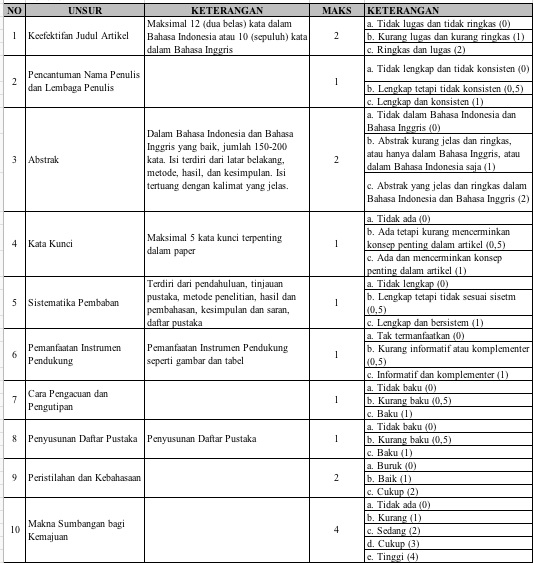
\includegraphics[width=1\textwidth]
      {figures/form1}}
      \caption{Form nilai bagian 1.}
      \label{form1}
      \end{figure}

	\begin{figure}[ht]
	      \centerline{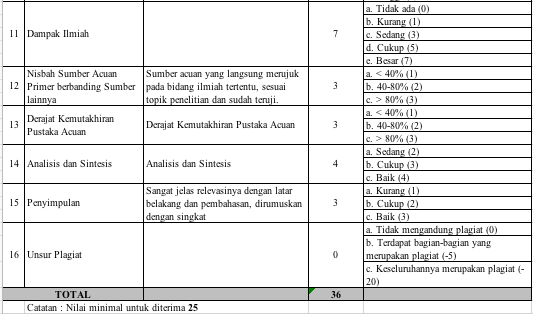
\includegraphics[width=1\textwidth]
	      {figures/form2}}
	      \caption{form nilai bagian 2.}
	      \label{form2}
	      \end{figure}

\chapter{FAQ}

M : Kalo Intership II atau TA harus buat aplikasi ?
D : Ga harus buat aplikasi tapi harus ngoding

M : Pa saya bingung mau ngapain, saya juga bingung mau presentasi apa?
D : Makanya baca de, buka jurnal topik `ganteng' nah kamu baca dulu sehari 5 kali ya, 4 hari udah 20 tuh. Bingung itu tanda kurang wawasan alias kurang baca.

M : Pa saya sudah cari jurnal terindeks scopus tapi ga nemu.
D : Kamu punya mata de? coba dicolok dulu. Kamu udah lakuin apa aja? tolong di list laporkan ke grup Tingkat Akhir. Tinggal buka google scholar klik dari tahun 2014, cek nama jurnalnya di scimagojr.com beres.

M : Pa saya belum dapat tempat intership, jadi ga tau mau presentasi apa?
D : kamu kok ga nyambung, yang dipresentasikan itu yang kamu baca bukan yang akan kamu lakukan.

M : Pa ini jurnal harus yang terindex scopus ga bisa yang lain ?
D : Index scopus menandakan artikel tersebut dalam standar semantik yang mudah dipahami dan dibaca serta bukan artikel asal jadi. Jika diluar scopus biasanya lebih sukar untuk dibaca dan dipahami karena tidak adanya proses review yang baik dan benar terhadap artikel.

M : Pa saya tidak mengerti
D : Coba lihat standar alasan

M : Pa saya bingung
D : Coba lihat standar alasan

M : Pa saya sibuk
D : Mbahmu....

M : Pa saya ganteng
D : Ndasmu....

M : Pa saya kece
D : wes karepmu lah....


Biasanya anda memiliki alasan tertentu jika menghadapi kendala saat proses bimbingan, disini saya akan melakukan standar alasan agar persepsi yang diterima sama dan tidak salah kaprah. Penggunaan kata alasan tersebut antara lain :

1. Tidak Mengerti : anda boleh menggunakan alasan ini jika anda sudah melakukan tahapan membaca dan meresumekan 15 jurnal. Sudah mencoba dan mempraktekkan teorinya dengan mencari di youtube dan google minimal 6 jam sehari selama 3 hari berturut-turut.

2. Bingung : anda boleh mengatakan alasan bingung setelah maksimal dalam berusaha menyelesaikan tugas bimbingan dari dosen(sudah dilakukan semua). Anda belum bisa mengatakan alasan bingung jika anda masih belum menyelesaikan tugas bimbingan dan poin nomor 1 diatas. Setelah anda menyelesaikan tugas bimbingan secara maksimal dan tahap 1 poin diatas, tapi anda masih tetap bingung maka anda boleh memakai alasan ini.

%next line adds the Bibliography to the contents page
\addcontentsline{toc}{chapter}{Bibliography}
%uncomment next line to change bibliography name to references
%\renewcommand{\bibname}{References}
\bibliography{references}        %use a bibtex bibliography file refs.bib
\bibliographystyle{plain}  %use the plain bibliography style

\end{document}

